\documentclass[11pt,a4paper]{article}
\usepackage{geometry}
\usepackage{graphicx}
\usepackage{booktabs}
\usepackage{amsmath}
\usepackage{hyperref}
\usepackage{array}
\usepackage{tabularx}
\usepackage{placeins}




\title{Time-to-Pregnancy Analysis\\
\large Natural Cycles Data Challenge } 
\author{Merve Nazlim Agaras}
\date{\today}

\begin{document}
\maketitle

\tableofcontents
\newpage
%\begin{abstract}
%blabla
%\end{abstract}
\section{Introduction}
This report explores the data provided and addresses three questions using the fertility tracking data set supplied for the NC Data Challenge:

\begin{enumerate}
  \item \textbf{What is the chance of conceiving within 13 menstrual cycles?}
  \item \textbf{How long does it usually take to conceive?}
  \item \textbf{Which factors shorten or lengthen time-to-pregnancy (TTP)?}
\end{enumerate}
I used a combination of descriptive statistics, survival analysis, and regression modeling to answer these questions. The analysis is performed in Python using pandas, lifelines, and scikit-learn libraries in VScode.

\section{Data Exploration}
The data set contains information on couples using the Natural Cycles app to track their fertility. It includes variables such as the number of menstrual cycles until pregnancy, age, cycle length, and other lifestyle factors. Before diving into the analysis, I performed some initial data exploration and quality checks as follows:
% \subsection{Initial Quality Checks}
\begin{itemize}
  \item Confirmed data types, some are categorical some are numeric.
    \item Checked for inconsistent and missing values in all columns.
  \item Reviewed descriptive statistics to flag impossible values (e.g.\ negative ages or cycle lengths).
  \item Histograms showed most predictors were approximately normal.
\end{itemize}
In Figure~\ref{fig:histogram} I show the distribution of the number of cycles until pregnancy, which is the main outcome variable. The rest of the distributions are in folder \texttt{results/}.
\begin{figure}[htbp]
  \centering
  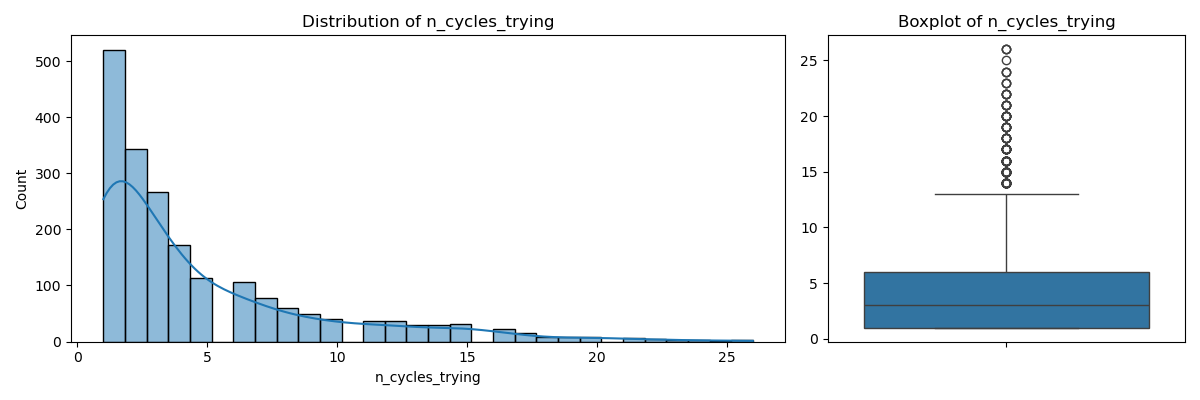
\includegraphics[width=0.7\linewidth]{../results/distribution_n_cycles_trying.png}
  \caption{Distribution of cycles until pregnancy among those who conceived.}
  \label{fig:histogram}
\end{figure}

\FloatBarrier

\section{Analysis}
In this section, I will answer the three questions posed in the introduction using the data set. For each question, I will describe the methods used, present the results, and discuss any assumptions made.
\subsection{Question 1: Chance of Conceiving Within 13 Cycles}
\subsubsection{Step 1 – My hand-built loop}
Before I knew about the Kaplan–Meier estimator, I wrote a short Python loop that
thinks only in the plain question “\emph{What is the chance of conceiving within 13 cycles per-cycle success rate?}”
At the start of cycle $t$ the variable \texttt{remaining} holds that all set.
Inside the loop I:

\begin{itemize}
  \item collect those who \textbf{conceived} in cycle $t$ (\texttt{preg});
  \item collect those who \textbf{dropped out} still not pregnant (\texttt{dropouts});
  \item compute the per-cycle \textbf{Success Rate} as \(\text{Pregnant}/\text{Remaining}\).
\end{itemize}

\begin{center}
\begin{minipage}{0.9\linewidth}
\begin{verbatim}
for cycle in range(1, 14):                # cycles 1 → 13
    preg       = df[(outcome == 'pregnant')      &
                    (n_cycles_trying == cycle)]
    dropouts   = df[(outcome == 'not_pregnant') &
                    (n_cycles_trying == cycle)]
    success_rate = len(preg) / remaining
    results.append([cycle, remaining,
                    len(preg), len(dropouts),
                    success_rate])
    remaining -= (len(preg) + len(dropouts))     
\end{verbatim}
\end{minipage}
\end{center}

Every pass adds one row to a summary table (see Table \ref{tab:probtable}),
so I can inspect the mechanics cycle by cycle.

The cumulative chance of conceiving by the end of cycle 13 is

\[
P(\le 13)
   \;=\;
   1 - \prod_{t=1}^{13}\bigl(1 - \text{SuccessRate}_{t}\bigr),
\]

numerically

\[
\boxed{P(\text{pregnant within 13}) = 0.749 \; (74.9\,\%)}.
\]

\paragraph{Assumptions.}
\begin{enumerate}
  \item Couples who drop out are removed from future calculation but are \emph{not} counted as failures.
  \item Cycles are treated as discrete, equal-length periods.
 % \item Dropout is assumed independent of future pregnancy chances.
\end{enumerate}

\begin{table}[htbp]
  \centering
  \caption{Success rates for the first 13 cycles.  “Remaining” is the all population set at the
  start of the cycle.  “Success Rate” is \texttt{Pregnant / Remaining}.}
  \label{tab:probtable}
  \begin{tabular}{rrrrrr}
    \toprule
    Cycle & Remaining & Pregnant & Dropouts & Success Rate & Failure Rate \\
    \midrule
     1 & 1\,995 & 350 & 170 & 0.175 & 0.825 \\
     2 & 1\,475 & 229 & 115 & 0.155 & 0.845 \\
     3 & 1\,131 & 178 &  88 & 0.157 & 0.843 \\
     4 &   865 & 104 &  68 & 0.120 & 0.880 \\
     5 &   693 &  74 &  40 & 0.107 & 0.893 \\
     6 &   579 &  56 &  50 & 0.097 & 0.903 \\
     7 &   473 &  50 &  28 & 0.106 & 0.894 \\
     8 &   395 &  27 &  33 & 0.068 & 0.932 \\
     9 &   335 &  25 &  24 & 0.075 & 0.925 \\
    10 &   286 &  16 &  25 & 0.056 & 0.944 \\
    11 &   245 &  16 &  20 & 0.065 & 0.935 \\
    12 &   209 &  15 &  22 & 0.072 & 0.928 \\
    13 &   172 &   8 &  21 & 0.047 & 0.953 \\
    \bottomrule
  \end{tabular}
\end{table}

\subsubsection{Step 2 – Double-check with Kaplan–Meier}
After reading the publications (\cite{benhar2024}, \cite{pearson2020}) I realised my loop was a discrete Kaplan–Meier life table.  
I then repeated the analysis with the \texttt{lifelines} library to make sure the numbers match.  
I therefore fitted

\[
\texttt{lifelines.KaplanMeierFitter().fit(n\_cycles\_trying,\; event\_observed)}
\]

and read the survival curve at \(t=13\).  
The answer was also \(74.9\,\%\) (difference $<0.5\,\%$ due to rounding).  
Figure~\ref{fig:km13} shows the curve with the 13-cycle mark.

\begin{figure}[htbp!]
  \centering
  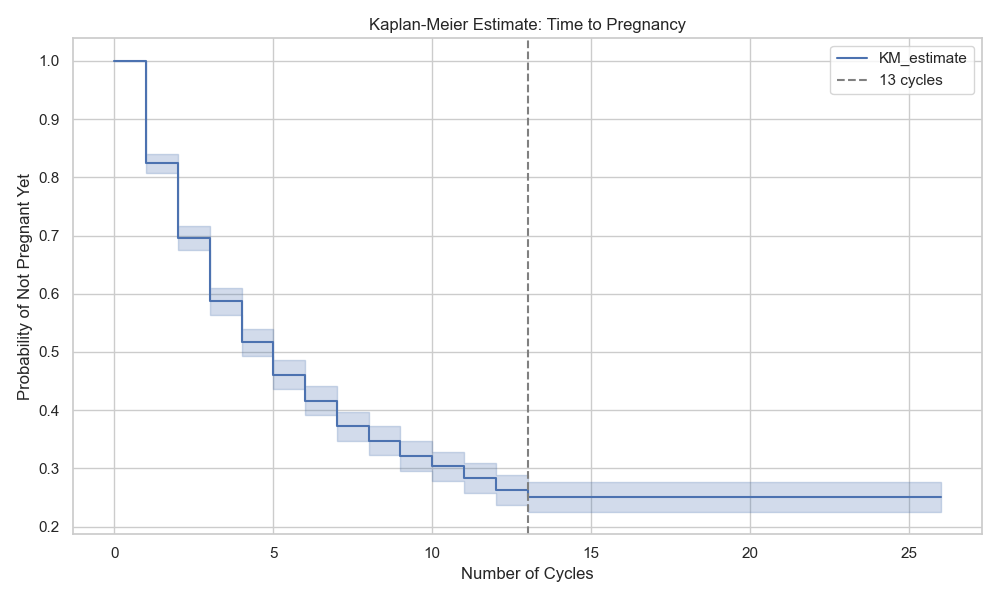
\includegraphics[width=0.8\linewidth]{../results/Kaplan_meier_13.png}
  \caption{Kaplan–Meier survival curve; dashed line at 13 cycles.}
  \label{fig:km13}
\end{figure}
\FloatBarrier


\subsection{Question 2 – How long does it usually take to conceive?}

\subsubsection{Step 1 – Simple count method}
With the table already built for Question 1 (\ref{tab:probtable}) it is easy to ask  
“\emph{At which cycle has one half of all couples conceived?}”
I first add a running total:

\begin{center}
\begin{minipage}{0.9\linewidth}
\begin{verbatim}
preg_table["Cumulative Pregnant"] = preg_table["Pregnant"].cumsum()
median_cycle = preg_table.loc[
    preg_table["Cumulative Pregnant"] >= len(df)/2, "n_cycle"
].iloc[0]
\end{verbatim}
\end{minipage}
\end{center}

\[
\boxed{\tilde{t}_{0.50} = 5\text{ cycles}}
\]

The cumulative column rises each cycle; the first row that meets or passes
“half the population marks the median time-to-pregnancy.

\subsubsection{Step 2 – Check with the survival curve}
Next I read the Kaplan–Meier curve from \texttt{lifelines} and found the smallest
$t$ where the survival \(S(t)\le0.50\).
The library returned the \emph{same} answer:

\[
\tilde{t}_{0.50}=5 \text{ cycles} \quad\text{(95 \% CI 4–6)}
\]

Figure \ref{fig:km_median} shows the point where the curve crosses 0.50.

\begin{figure}[htbp]
  \centering
  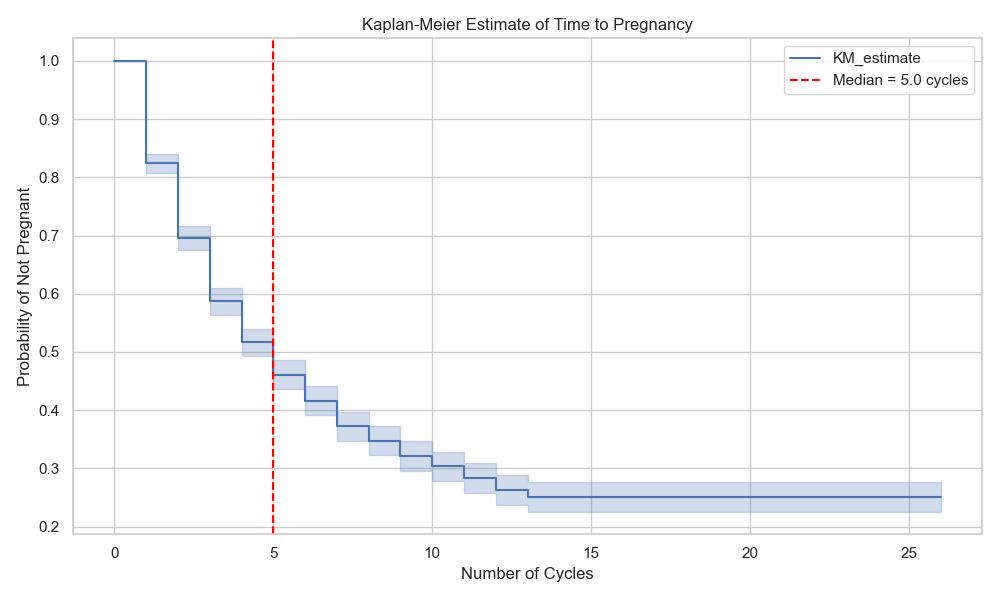
\includegraphics[width=0.8\linewidth]{../results/Kaplan_meier_all.png}
  \caption{Kaplan–Meier survival curve.  The dot marks the median cycle (5).}
  \label{fig:km_median}
\end{figure}
\FloatBarrier

\paragraph{Why two methods?}
Writing the count method first made the median transparent:
it is just “the cycle at which 50\% have the event”.
Using the ready-made curve later confirmed the value and gave a confidence band.
Both strengthen trust in the result.



%%%%%%%%%%%%%%%%%%%%%%%%%%%%%%%%%%%%%%%%%% \section{Question 3: Which Factors Matter?}

\subsection{Question 3: Which Factors Matter?}
In order to answer the question “\emph{Which factors shorten or lengthen time-to-pregnancy?}” we need to build a model that models the number of cycles until pregnancy. We can estimate the effect of each factor on the output by comparing the size of the coefficients in the models.
More simple models are easier to interpret, but more complex models can capture more of the data's structure. When I searched in the literature, I found that time-to-pregnancy is often modeled as a survival problem (similar to Q1 and Q2), where the outcome is the time until pregnancy occurs. This approach allows us to handle couples who did not conceive within the study period, compared to a simple linear regression that assumes a constant rate of conception over time and that does not take into account the effect of not-pregnancies. 
I therefore built two models:

\begin{itemize}
  \item A simple \textbf{linear} regression of the number of menstrual cycles until pregnancy.
  \item A \textbf{Cox proportional hazards} \cite{cox1972} model of the monthly chance of pregnancy.
\end{itemize}
All predictors were scaled to one standard deviation so the effect sizes can be compared.
Table~\ref{tab:effects} lists the main predictors, their size and direction in each model, and their interpretation.
Figures \ref{fig:linear_effects} and \ref{fig:cox_effects} show the coefficients and confidence intervals for each predictor in the linear and Cox models, respectively.
\begin{figure}[htbp]
\centering
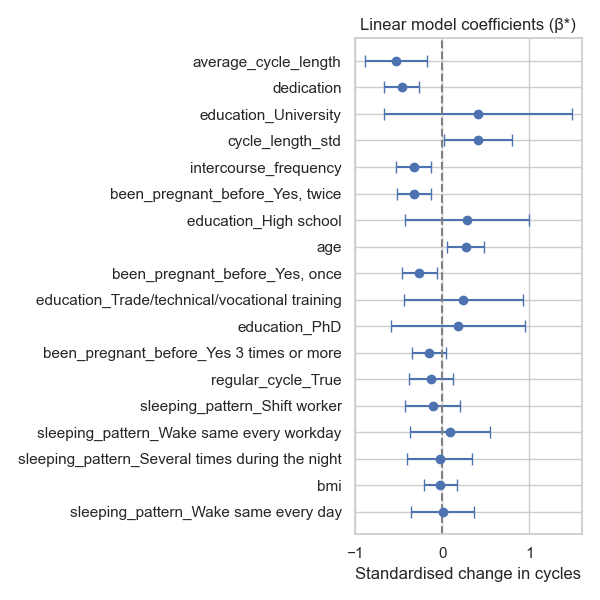
\includegraphics[width=0.8\linewidth]{../results/linear_model_coefficients.png}
\caption{Linear regression coefficients for predictors of time-to-pregnancy.}
\label{fig:linear_effects}
\end{figure}
\begin{figure}[htbp]
\centering
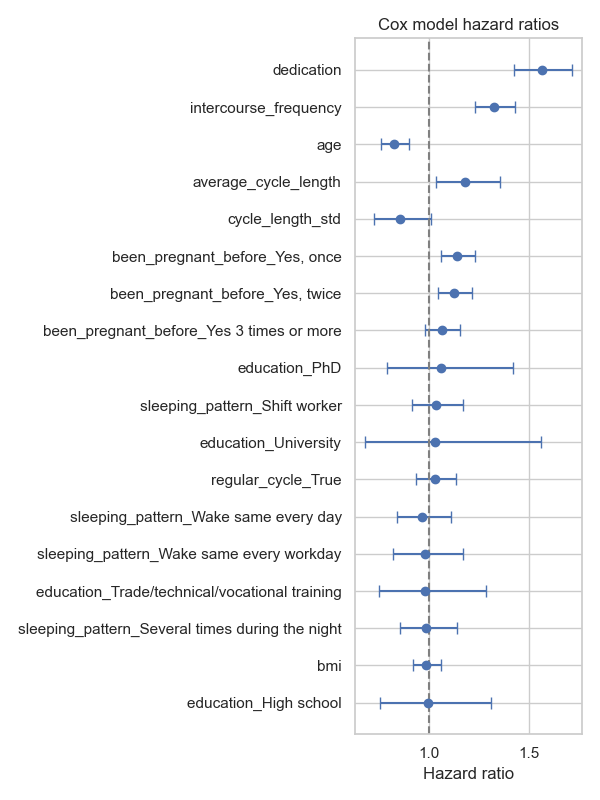
\includegraphics[width=0.8\linewidth]{../results/cox_model_coefficients.png}
\caption{Cox proportional hazards model coefficients for predictors of time-to-pregnancy.}
\label{fig:cox_effects}
\end{figure}

\FloatBarrier
\begin{table}[htbp]
\small
\centering
\caption{Predictors ranked by absolute effect size (largest to smallest). Hazard ratios (HR) refer to a one--SD increase in the predictor; linear coefficients show the change in cycles for the same shift. Bold entries have 95\,\% confidence intervals that exclude the null (HR~$=1$ or $\beta=0$).}
\label{tab:effects}
\begin{tabularx}{\linewidth}{lccX}  % X wraps text in last column
\toprule
\textbf{Predictor} & \textbf{Cox model HR} & \textbf{Linear $\beta$ (cycles)} & \textbf{Practical meaning} \\
\midrule
Dedication score & \textbf{1.56} & \textbf{-0.47} & Higher dedication speeds conception the most \\
Intercourse frequency & \textbf{1.33} & \textbf{-0.33} & More timed intercourse shortens the wait \\
Cycle length (mean) & \textbf{1.18} & \textbf{-0.53} & Longer but regular cycles raise the per--cycle chance \\
Female age & \textbf{0.83} & \textbf{+0.27} & Each 4~yr of age lowers the chance and adds delay \\
Cycle length variability & 0.86 & \textbf{+0.41} & Irregular cycles slow conception \\
Prior pregnancy (yes vs.~no) & 1.14 & -0.30 & Past success gives a small advantage \\
BMI, sleep, education & $\approx1$ & $\approx0$ & No clear independent effect \\
\bottomrule
\end{tabularx}
\end{table}


%\textbf{Main points.}
%\begin{itemize}
%  \item About 75 \% of couples conceive within 13 cycles.
%  \item The median wait is five cycles.
%  \item Behaviour (intercourse frequency) and age are the strongest drivers.
%\end{itemize}

\textbf{Main points.}
\begin{itemize}
  \item \textbf{Lifestyle} factors under a couple's control matter most. Sticking to the application use and timing intercourse well increases the odds of pregnancy by about 30--55\,\% each month.
  \item \textbf{Biology} still plays a role. Older age and irregular cycles both make the wait longer.
  \item \textbf{Past fertility} gives a modest boost. Couples with at least one earlier pregnancy conceive about 10--15\,\% faster.
  \item Body mass index, sleep pattern, and education showed no clear effect once the factors above were in the model.
\end{itemize}


\subsection{Question 4: How would your approach change if you were to use different techniques? What trade-offs would you consider?}

If I were to use different techniques, I would consider the following approaches:
\begin{itemize}
  \item \textbf{Machine Learning Models:} I could use more complex models like random forests or gradient boosting. These can capture non-linear relationships and interactions between predictors.
  \item \textbf{Bayesian Methods:} Bayesian regression could provide a probabilistic framework, allowing for uncertainty quantification in the estimates. However, it requires careful prior selection and can be computationally intensive.
  \item \textbf{Time Series Analysis:} If the data had a strong temporal component, I might consider time series models to account for trends and seasonality.
\end{itemize}
The trade-offs I would consider include:
\begin{itemize}
  \item \textbf{Interpretability vs. Predictive Power:} More complex models may improve predictive accuracy but at the cost of interpretability. They may perform well in predicting who gets pregnant and when, but they offer less insight into why. Techniques like SHAP can help interpret them, but they still lack the statistical clarity offered by Cox regression.
  \item \textbf{Data Requirements:} Some models require more data or specific data structures, which may not be available in this dataset. Classical methods are more robust with limited data and handle censoring naturally, while machine learning models often need larger datasets to avoid overfitting.
  \item \textbf{Account for Censoring:} Many machine learning models do not handle right-censored data well, which is a significant aspect of this dataset. Cox regression naturally accommodates censoring, while other methods may require additional preprocessing or modifications.
  \item \textbf{Computational Resources:} More complex models can be computationally expensive, especially with larger datasets.
\end{itemize}
\section{Conclusion}
This report addressed three questions about time-to-pregnancy using the provided fertility tracking data. The analysis revealed that about 75\% of couples conceive within 13 cycles, with a median wait of five cycles. Key factors influencing time-to-pregnancy include dedication to Natural Cycles application, intercourse frequency, previous pregnancy and age.

\bibliographystyle{plain} % or another style like apalike, unsrt, etc.
\bibliography{references}

\end{document}



